\documentclass[journal]{IEEEtran}

\usepackage{iftex}
\ifPDFTeX
  \usepackage[T1]{fontenc}
\else
  \usepackage{fontspec}
  \setmainfont{Times New Roman}
  \DeclareFontShape{TU}{TimesNewRoman(0)}{m}{sc}{<-> ssub*TimesNewRoman(0)/m/n}{}
\fi
\usepackage{amsmath,amssymb,amsthm}
\usepackage{booktabs}
\usepackage{graphicx}
\usepackage{url}
\usepackage{array}
\usepackage{multirow}
\usepackage{algorithm}
\usepackage{algpseudocode}

\newtheorem{proposition}{Proposition}

\title{Drift-Triggered Conformal Quality Gating for Industrial IoT under Production Shift}

\author{Siqiang Zhao and Fengxiang Zhang%
\thanks{S. Zhao is the corresponding author and is with Toulouse INP, Toulouse, France, and Sichuan University--Pittsburgh Institute, Sichuan University, Chengdu, China (e-mail: siqiang.zhao@etu.toulouse-inp.fr; ORCID: 0009-0008-5758-7929). F. Zhang is with Southwest Jiaotong University, Chengdu, Sichuan, China (e-mail: zfengxiang309@gmail.com).}}

\begin{document}
\maketitle

\begin{abstract}
Industrial quality models are often validated on a historical regime and then used during production ramp-up, when product mix, equipment, suppliers, or operating rate may change. We present a drift-triggered conformal quality gate (DTCG) for industrial Internet-of-Things deployments. DTCG couples an unlabeled batch-shift detector, class-conditional conformal calibration, a first-shift inspection hold, delayed-label rolling recalibration, and a traceable decision event. Chronological experiments use two public manufacturing benchmarks: UCI SECOM and AI4I 2020 Predictive Maintenance. On SECOM, a probability threshold and global conformal calibration miss 81.3\% and 79.5\% of failures, while class-conditional CP and DTCG miss 3.3\% and inspect 80.8\% and 82.0\% of units, respectively. On AI4I, DTCG obtains 10.1\% missed failures and 11.1\% inspection. Five component ablations, sensitivity sweeps, paired Wilcoxon tests, and a stable-prefix stress test show that DTCG's main value is policy-level: it converts drift evidence into a conservative first action and an auditable delayed-label state transition. These are empirical results on public proxies, not a claim of Airbus or post-shift distribution-free validity.
\end{abstract}

\begin{IEEEkeywords}
industrial Internet of Things, conformal prediction, distribution shift, quality inspection, digital thread
\end{IEEEkeywords}

\section{Introduction}
\label{sec:intro}

Industrial AI increasingly sits between a sensor observation and a manufacturing decision. In a quality workflow, the relevant question is not only whether a classifier is accurate on a held-out static set. It is whether a unit or lot can be released automatically, or whether engineering inspection should be requested, when the process is changing and the true label is delayed. This distinction is central to aerospace-oriented production ramp-up, where a model may encounter new product variants, equipment states, supplier streams, or production rates. The industrial motivation is consistent with the broader aerospace digital-thread problem: manufacturing, inspection, maintenance, and service information must be connected over the product life cycle \cite{airbus2024report,eskue2023}. The manuscript is also aligned with the stated scope of \emph{IEEE Transactions on Industrial Informatics}, which includes AI-enabled industrial automation, industrial cyber--physical systems, and IIoT applications \cite{tii_scope}.

Let $X$ denote an industrial sensor snapshot and $Y\in\{0,1\}$ denote a failure or nonconformance outcome. A model trained on an earlier regime estimates $p(x)=\Pr(Y=1\mid X=x)$. If the marginal distribution of $X$ changes, a calibration sample may no longer describe the stream at deployment. Concept drift and nonstationary learning are established problems for evolving data streams \cite{gama2014,lu2019,ditzler2015}. Under class imbalance, an apparently favorable overall accuracy can coexist with a large conditional missed-failure rate. A confidence score without a decision policy is therefore incomplete: the system must specify when it will stop auto-release, how it will use inspection labels that arrive later, and how a reviewer can reconstruct why a decision was made.

Conformal prediction (CP) provides model-agnostic prediction sets and finite-sample coverage under exchangeability \cite{vovk2005,shafer2008,lei2018,angelopoulos2023}. Weighted CP addresses covariate shift when a density ratio is known or accurately estimated \cite{tibshirani2019}; adaptive methods address online distribution changes \cite{gibbs2021,barber2021}. Recent work has studied CP for industrial time series under shift \cite{zhang2025} and out-of-distribution time-series classification \cite{nanopoulos2025}. However, these ingredients do not by themselves define a release gate with an inspection budget, a first-shift safety action, delayed-label rules, and a quality-system audit record.

This paper addresses that decision-layer gap. We make five contributions:
\begin{enumerate}
    \item We define DTCG, which couples an unlabeled batch drift score to an asymmetric class-conditional conformal release rule and a human inspection policy.
    \item We specify a delayed-label protocol: the first shifted batch is held for inspection, and only outcomes already available from inspected batches can update rolling calibration.
    \item We give a finite-sample pre-shift proposition and a proof, while explicitly separating it from any post-shift guarantee.
    \item We define and export a batch-level digital-thread event containing the model, calibration, drift, threshold, decision, and escalation state.
    \item We evaluate two public manufacturing benchmarks with ablations, parameter sensitivities, paired statistical tests, and a controlled stable-prefix/sudden-shift detector test.
\end{enumerate}

The paper is aerospace-oriented but not an Airbus-data paper. SECOM is a semiconductor manufacturing benchmark, and AI4I is a predictive-maintenance benchmark described by UCI as synthetic data reflecting industrial maintenance observations \cite{uci_secom,uci_ai4i}. This boundary is intentional: the study supports method development and an internship portfolio without implying access to proprietary Airbus data or aircraft-production validation.

\section{Related Work}
\label{sec:related}

\subsection{Industrial monitoring and quality inspection}
Data-driven process monitoring traditionally combines multivariate statistics, soft sensors, and machine-learning models to detect abnormal operation and diagnose faults \cite{qin2012,ge2017}. Reviews emphasize that industrial measurements are high-dimensional, correlated, incomplete, and affected by process modes. Classical online-stream methods such as adaptive windows and high-speed stream mining provide mechanisms for updating a model as data changes \cite{domingos2000,bifet2007}. More recent surveys organize the nonstationary-learning problem around drift detection, model adaptation, and evaluation under changing distributions \cite{gama2014,ditzler2015,lu2019}.

Quality inspection has also moved toward in-line automation and edge intelligence. Azamfirei \emph{et al.} review automation for zero-defect in-line inspection \cite{azamfirei2023}, while Hu \emph{et al.} describe a software-defined edge controller for IIoT product-quality inspection \cite{hu2023}. Rodríguez \emph{et al.} find that IIoT anomaly-classification research remains less mature than anomaly detection and that contextual information is often underused \cite{rodriguez2023}. A systematic review of CPS/IoT data quality identifies sensor failures, incomplete records, and uncertain operating environments as recurring sources of decision risk \cite{goknil2023}. These works motivate an edge-compatible decision component, but they do not specify a distribution-free release rule coupled to delayed inspection outcomes.

\subsection{Distribution shift and drift detection}
Domain adaptation formalizes the challenge of learning across different source and target domains \cite{ben2010}. Dataset-shift studies compare two-sample tests, classifier-based detectors, and uncertainty signals; domain discriminators are useful because they can identify whether two feature samples are distinguishable even when labels are unavailable \cite{rabanser2019,ovadia2019}. Maximum mean discrepancy provides a kernel two-sample alternative with distribution-free testing results and quadratic, or approximated linear, computation \cite{gretton2012}. Score-based out-of-distribution detection provides a simple baseline for recognizing unfamiliar inputs \cite{hendrycks2017}; label-shift methods instead focus on changes in class proportions while holding conditional structure fixed \cite{lipton2018}.

DTCG chooses a cross-fitted domain classifier as a deliberately simple trigger. This is not a claim that domain AUC is a universal or causal drift measure. It is an unlabeled, batch-level signal that can be logged before inspection labels arrive. The operational novelty is what follows the signal: a controlled hold, a delayed-label update rule, and an explicit state in the quality record. The controlled stable-prefix experiment in Section~\ref{sec:results} tests whether the trigger can remain quiet when the observed features are calibration-like and respond after a sudden feature change.

\subsection{Conformal uncertainty and delayed labels}
The conformal framework turns a nonconformity score into a prediction region with an explicit error level under exchangeability \cite{vovk2005,shafer2008,angelopoulos2023}. Class-conditional or Mondrian constructions condition calibration on a pre-response category; the original Mondrian formulation is grounded in the algorithmic-learning framework of Vovk \emph{et al.}, while Mondrian conformal regressors provide a direct modern reference for this structure \cite{vovk2005,bostrom2020}. Conformalized quantile regression and jackknife+ improve efficiency in other predictive-inference settings \cite{romano2019,barber2021}. Under covariate shift, weighted CP estimates the target density ratio from unlabeled covariates \cite{tibshirani2019}. Adaptive conformal inference allows the data-generating distribution to vary over time \cite{gibbs2021}.

The closest industrial work to this paper is Zhang and Zhou's uncertainty quantification for industrial time series with distribution shift \cite{zhang2025}; Nanopoulos and Buza study CP for out-of-distribution time-series classification \cite{nanopoulos2025}. We differ in the target abstraction. Their primary object is an uncertainty or prediction-set procedure, whereas our object is a release-versus-inspection gate with an operational capacity cost and a trace record. We use class-conditional CP as the safety layer, but do not claim a new CP theorem. The delayed-label protocol is related to online learning with delayed feedback \cite{joulani2016} and recent online continual-learning work that makes label latency explicit \cite{botos2024}. Active learning similarly treats human labeling as a resource to be queried strategically \cite{settles2009}; DTCG uses inspection as a safety escalation rather than optimizing an active-learning acquisition function.

\subsection{Digital thread and traceability}
Digital-thread roadmaps for aerospace components emphasize data capture across design, manufacture, test, inspection, and life-cycle monitoring, while also noting that complete thread connections are not consistently deployed \cite{eskue2023}. Component digital threads can be extended with identity and material-passport concepts \cite{paramatmuni2023}. DTCG contributes a narrow but implementable record at the AI decision boundary: the model and calibration versions, drift evidence, threshold, decision, and escalation reason are stored together. This makes the AI decision linkable to a future MES/QMS record without requiring a new enterprise architecture.

\section{Problem Setting and Requirements}
\label{sec:setting}

\subsection{Operational requirements}
We model a production line in which an IIoT gateway receives a feature vector for each unit or lot. A quality model may recommend automatic release, but a quality engineer remains the authority for non-routine or uncertain cases. The system has four requirements:
\begin{itemize}
    \item \textbf{Asymmetric risk:} a missed failure is more costly than an additional inspection, so evaluation must report the conditional missed-failure rate.
    \item \textbf{Unlabeled drift detection:} inspection outcomes arrive after the release decision, so the shift monitor must operate on the current batch before labels are available.
    \item \textbf{Delayed-label correctness:} current-batch labels cannot influence the threshold used to decide that same batch.
    \item \textbf{Traceability:} a reviewer must be able to reconstruct the model, calibration state, drift evidence, threshold, decision, and escalation reason.
\end{itemize}

\subsection{Decision and risk metrics}
For sample $t$, the predictor produces $p_t=f_{\theta}(x_t)$. The gate returns either $a_t=\mathrm{AUTO\text{-}RELEASE}$ or $a_t=\mathrm{INSPECT}$. The empirical missed-failure rate is
\begin{equation}
\widehat{r}_{\mathrm{miss}}=\frac{\sum_t \mathbb{1}\{a_t=\mathrm{AUTO\text{-}RELEASE},y_t=1\}}{\sum_t \mathbb{1}\{y_t=1\}}.
\label{eq:miss}
\end{equation}
The efficiency metric is the auto-release rate $\widehat{e}=T^{-1}\sum_t\mathbb{1}\{a_t=\mathrm{AUTO\text{-}RELEASE}\}$. We also report inspection rate, failure capture, the model's ROC AUC and average precision, and batch-level state transitions. These metrics expose the safety--capacity trade-off rather than hiding it in overall accuracy.

\section{Drift-Triggered Conformal Quality Gate}
\label{sec:method}

\subsection{Predictor and preprocessing}
The predictor can be replaced by any probabilistic classifier. We use a random forest so that the contribution is not tied to a deep architecture. The model, feature-retention mask, and imputation statistics are fitted only on the proper-training block. A fixed positive-class weight encodes the cost asymmetry before the chronological test period is evaluated.

\subsection{Class-conditional conformal threshold}
Let $\mathcal{C}_0=\{p_i:y_i=0\}$ and $\mathcal{C}_1=\{1-p_i:y_i=1\}$ be calibration nonconformity scores for the pass and failure classes. For error level $\alpha$, let $Q_\alpha(\mathcal{C})$ be the order statistic at rank
\[
 r_\alpha(\mathcal{C})=\left\lceil(|\mathcal{C}|+1)(1-\alpha)\right\rceil.
\]
For example, when $|\mathcal{C}|=400$ and $\alpha=0.10$, the rank is $\lceil401\times0.90\rceil=361$. This finite-sample correction is the reason the quantile is not simply the empirical 90th percentile; under exchangeability it gives the usual marginal noncoverage bound $\Pr\{Y\notin\Gamma(X)\}\leq\alpha$ for the conformal prediction set.

We define the one-sided class-conditional release threshold
\begin{equation}
\tau_{\mathrm{MC}}=\min\left\{Q_\alpha(\mathcal{C}_0),1-Q_\alpha(\mathcal{C}_1)\right\}.
\label{eq:tau}
\end{equation}
The auto-release rule is $p_t<\tau_{\mathrm{MC}}$; otherwise the unit is routed to inspection. Both terms must be satisfied: the score is sufficiently pass-like and sufficiently unlike the failure class.

\begin{proposition}[Pre-shift failure noncoverage]
\label{prop:pre-shift}
Assume that the predictor is fixed independently of calibration data and that the calibration failure scores in $\mathcal{C}_1$ and a future failure score $1-p(X)$ are exchangeable conditional on $Y=1$. Then the class-conditional release rule in (\ref{eq:tau}) satisfies
\begin{equation}
\Pr\left\{p(X)<\tau_{\mathrm{MC}}\mid Y=1\right\}\leq\alpha.
\label{eq:prop}
\end{equation}
\end{proposition}

\begin{proof}
If $p(X)<\tau_{\mathrm{MC}}$, then $p(X)<1-Q_\alpha(\mathcal{C}_1)$ and hence $1-p(X)>Q_\alpha(\mathcal{C}_1)$. The future failure score is exchangeable with the $|\mathcal{C}_1|$ calibration failure scores. The order-statistic rank defined above leaves at most an $\alpha$ fraction of the $|\mathcal{C}_1|+1$ exchangeable ranks above the threshold. Therefore the conditional probability of a failure score exceeding $Q_\alpha(\mathcal{C}_1)$ is at most $\alpha$, which proves (\ref{eq:prop}).
\end{proof}

This proposition bounds auto-release among failures, not the posterior probability $\Pr(Y=1\mid p(X)<\tau)$, and it applies only to the stated pre-shift exchangeability condition. Once the stream changes, DTCG does not claim that this bound survives automatically.

\subsection{Unlabeled batch drift score}
At the beginning of batch $b$, the current feature matrix $X_b$ is available but $Y_b$ is not. We concatenate calibration features $X_{\mathrm{cal}}$ and current features $X_b$, assign domain labels $d=0$ and $d=1$, and fit a standardized logistic domain classifier. Its three-fold cross-fitted ROC AUC is
\begin{equation}
A_b=\mathrm{AUC}\left(\widehat{h}_{-k}(X_{\mathrm{cal}}\cup X_b),d\right).
\label{eq:auc}
\end{equation}
We flag a batch when $A_b\geq\gamma$, with $\gamma=0.65$ fixed before testing. A high AUC means that the two feature domains are distinguishable; it does not identify the physical cause or prove label shift. The detector is consequently treated as evidence for escalation, not as a safety certificate.

\subsection{Stateful gate policy}
The gate maintains $s_b$, indicating whether a shift has already been observed, and $\mathcal{L}_b$, containing labels from completed inspections. The state machine is: stable $\rightarrow$ first-shift-hold $\rightarrow$ shifted-base-calibration $\rightarrow$ shifted-rolling-calibration. The first-shift state is entered only once per run. A rolling state is allowed only after at least $m=5$ inspected failures are available. The decision order is summarized in Algorithm~\ref{alg:dtcg}.

\begin{algorithm}[t]
\caption{DTCG gate policy.}
\label{alg:dtcg}
\begin{algorithmic}[1]
\Require Current batch $X_b$, predictor $f_\theta$, calibration scores, $\alpha$, $\gamma$, minimum $m$
\State Compute $p_b=f_\theta(X_b)$ and the unlabeled domain AUC $A_b$
\If{$A_b<\gamma$}
    \State Set $\tau_b=\tau_{\mathrm{MC}}$ and record \textit{stable}
\ElsIf{no shift has been seen}
    \State Set $\tau_b=0$, inspect all units, record \textit{first-shift-hold}
\ElsIf{at least $m$ prior inspected failures are available}
    \State Compute $\tau_{\mathrm{rolling}}$ and set $\tau_b=\min(\tau_{\mathrm{MC}},\tau_{\mathrm{rolling}})$
    \State Record \textit{shifted-rolling-calibration}
\Else
    \State Set $\tau_b=\tau_{\mathrm{MC}}$ and record \textit{shifted-base-calibration}
\EndIf
\State Decide \textsc{Auto-Release} iff $p_b<\tau_b$; append inspected labels only after all decisions
\end{algorithmic}
\end{algorithm}

The first-shift hold is intentionally expensive: it trades one batch of release efficiency for verified outcomes and a defensible state transition. The minimum $m$ is an engineering guardrail, not a universal optimum. In a real line it should be selected from the inspection capacity, cost matrix, and minimum detectable failure count.

\subsection{Audit event}
For every batch, the service emits
\begin{equation*}
\begin{gathered}
\langle\texttt{lot\_id},\texttt{model\_version},\texttt{calibration\_version},\\
\texttt{policy\_version},A_b,\texttt{gate\_mode},\tau_b,\texttt{decision}\rangle.
\end{gathered}
\end{equation*}
The exported study trace additionally stores action counts, the shift flag, and failures observed among inspected units. A production MES/QMS integration should add timestamps, process/equipment identifiers, source-data hashes, nonconformance identifiers, and human disposition links. The audit event is metadata-only and need not replicate raw sensor data.

\section{Experimental Protocol}
\label{sec:experiments}

\subsection{Datasets and chronological splits}
Table~\ref{tab:data} summarizes the two public benchmarks. SECOM contains 1,567 semiconductor-manufacturing records, 590 raw process features, timestamps, missing values, and 104 failures \cite{uci_secom}. AI4I contains 10,000 records and 14 raw columns for predictive maintenance; its UCI description identifies it as synthetic data reflecting industrial maintenance observations \cite{uci_ai4i}. We use AI4I as a second industrial validation, not as an aircraft-quality dataset.

\begin{table}[t]
\centering
\caption{Datasets and chronological protocol.}
\label{tab:data}
\small
\begin{tabular}{lrrrrr}
\toprule
Dataset & $N$ & Raw $d$ & Failures & Train & Cal/Test \\
\midrule
SECOM & 1,567 & 590 & 104 & 400 & 400/767 \\
AI4I & 10,000 & 14 & 339 & 6,000 & 2,000/2,000 \\
\bottomrule
\end{tabular}
\end{table}

Rows preserve the supplied order; SECOM also supplies timestamps that are consistent with the chronological interpretation. The first block fits the model and all preprocessing, the second block calibrates thresholds, and the final block is tested in chronological batches. SECOM retains 574 features after a training-only observed-value filter. AI4I drops identifiers and failure-mode subtype columns to prevent target leakage, maps the product type to fixed one-hot features, and retains eight predictors. No test label is used to select a threshold, hyperparameter, drift trigger, or policy variant.

\subsection{Methods and implementation}
The common predictor is a random forest with 500 trees, square-root feature subsampling, minimum leaf size two, and class weights $w_0=1,w_1=8$. The baselines are:
\begin{itemize}
    \item \textbf{Probability-0.5:} auto-release when $p_t<0.5$.
    \item \textbf{Global-CP:} one pooled conformal threshold.
    \item \textbf{Mondrian-CP:} the class-conditional threshold in (\ref{eq:tau}); this is the static baseline.
    \item \textbf{Weighted-Mondrian:} unlabeled domain-classifier density-ratio weighting of the two class-specific calibration sets.
    \item \textbf{Periodic-Rolling-CP:} update class-conditional calibration whenever at least five prior inspected failures exist, with no drift trigger.
    \item \textbf{DTCG-Proposed:} Algorithm 1 with $\alpha=0.10$, $\gamma=0.65$, batch size 50, $m=5$, and at most 200 recent inspected labels.
\end{itemize}

We evaluate five ablations: no first-shift hold, no rolling update, always rolling without a drift trigger, and minimum inspected-failure values $m=1$ and $m=10$. Sensitivity experiments independently sweep $\alpha\in\{0.05,0.10,0.15,0.20\}$, $\gamma\in\{0.55,0.60,0.65,0.70,0.75\}$, batch size $\in\{25,50,75,100\}$, and class weight $w_1\in\{4,8,16,32\}$. All other settings remain at their defaults for each one-factor sweep. Five fixed seeds $\{7,17,27,37,47\}$ are used. The primary table aggregates 80 seed--batch evaluations for SECOM and 200 for AI4I; the statistical tests pair identical seed--batch coordinates.

\section{Results}
\label{sec:results}

\subsection{Main multi-dataset performance}
Table~\ref{tab:main} reports the main gate results. On SECOM, probability and global-CP baselines auto-release nearly everything and miss 81.3\% and 79.5\% of failures. Class-conditional CP reduces missed failures to 3.3\% while inspecting 80.8\% of units. DTCG has the same mean missed-failure rate, inspects 82.0\%, and auto-releases 18.0\%. On AI4I, the predictor is stronger and the operating point is less conservative: DTCG auto-releases 88.9\%, inspects 11.1\%, and has a 10.1\% mean missed-failure rate. This cross-dataset difference is a result, not a tuning error: it shows that the policy's safety--capacity trade-off depends on the data regime.

\begin{table*}[t]
\centering
\caption{Chronological quality-gate performance. Values are mean $\pm$ standard deviation over seed--batch evaluations. Missed failure is conditional on observed failures in a batch.}
\label{tab:main}
\small
\begin{tabular}{llccccc}
\toprule
Dataset & Method & Auto-release & Inspection & Missed failure & Failure capture & Mean $\tau$ \\
\midrule
\multirow{6}{*}{SECOM}
& Probability-0.5 & $100.0\pm0.0$\% & $0.0\pm0.0$\% & $81.3\pm39.3$\% & $0.0\pm0.0$\% & 0.500 \\
& Global-CP & $98.1\pm2.3$\% & $1.9\pm2.3$\% & $79.5\pm38.9$\% & $1.7\pm5.9$\% & 0.209 \\
& Weighted-Mondrian & $32.8\pm17.6$\% & $67.2\pm17.6$\% & $10.0\pm25.0$\% & $71.3\pm42.3$\% & 0.126 \\
& Periodic-Rolling-CP & $29.3\pm17.2$\% & $70.7\pm17.2$\% & $8.1\pm22.1$\% & $73.2\pm41.5$\% & 0.123 \\
& Mondrian-CP & $19.2\pm13.4$\% & $80.8\pm13.4$\% & $3.3\pm13.3$\% & $77.9\pm39.9$\% & 0.115 \\
& DTCG-Proposed & $18.0\pm14.0$\% & $82.0\pm14.0$\% & $3.3\pm13.3$\% & $77.9\pm39.9$\% & 0.108 \\
\midrule
\multirow{6}{*}{AI4I}
& Probability-0.5 & $98.8\pm1.8$\% & $1.2\pm1.8$\% & $30.1\pm40.9$\% & $29.9\pm40.8$\% & 0.500 \\
& Global-CP & $93.0\pm6.7$\% & $7.0\pm6.7$\% & $11.4\pm28.3$\% & $48.6\pm48.0$\% & 0.081 \\
& Weighted-Mondrian & $90.9\pm7.3$\% & $9.1\pm7.3$\% & $10.1\pm27.7$\% & $49.9\pm48.6$\% & 0.058 \\
& Periodic-Rolling-CP & $92.8\pm7.2$\% & $7.3\pm7.2$\% & $11.4\pm28.3$\% & $48.6\pm48.0$\% & 0.083 \\
& Mondrian-CP & $90.9\pm7.9$\% & $9.1\pm7.9$\% & $10.1\pm27.7$\% & $49.9\pm48.6$\% & 0.062 \\
& DTCG-Proposed & $88.9\pm16.2$\% & $11.1\pm16.2$\% & $10.1\pm27.7$\% & $49.9\pm48.6$\% & 0.060 \\
\bottomrule
\end{tabular}
\end{table*}

The common predictor has test ROC AUC $0.673\pm0.032$ and average precision $0.113\pm0.012$ on SECOM, versus $0.953\pm0.004$ and $0.690\pm0.006$ on AI4I. The gate therefore changes the operational behavior of a moderately discriminative model on SECOM, while AI4I shows that strong discrimination can reduce the inspection burden but does not eliminate the need to state the conditional risk.

\subsection{Ablation study and first-shift hold}
Table~\ref{tab:ablation} reports the component ablations. On SECOM, removing the first-shift hold increases auto-release from 18.0\% to 19.2\% and removes the only state transition that guarantees the first flagged batch is fully inspected. Removing rolling leaves the aggregate result at 18.0\% auto-release and 3.3\% missed failures because the base class-conditional threshold is already conservative. Always rolling increases auto-release to 29.3\% but raises missed failures to 8.1\%. Lowering $m$ to one and increasing it to ten both produce the same aggregate result as the proposed policy in this trace. On AI4I, removing the first hold raises auto-release from 88.9\% to 90.9\% but retains a 10.1\% missed-failure rate; always rolling reaches 92.8\% auto-release but misses 11.4\%. The first five batches contain five missed failures in the no-hold variant and also five in the proposed variant because the held first batch has one failure and later batches dominate the first-five total. The hold's measured benefit here is therefore procedural: it guarantees no automatic release in the first shifted batch, at a cost of 50 units per seed, rather than reducing the retrospective first-five count in this particular trace.

\begin{table*}[t]
\centering
\caption{DTCG ablations. Values are means over seed--batch evaluations.}
\label{tab:ablation}
\small
\begin{tabular}{llccc}
\toprule
Dataset & Variant & Auto-release & Inspection & Missed failure \\
\midrule
\multirow{6}{*}{SECOM}
& DTCG-Proposed & 18.0\% & 82.0\% & 3.3\% \\
& No first-shift hold & 19.2\% & 80.8\% & 3.3\% \\
& No rolling & 18.0\% & 82.0\% & 3.3\% \\
& Always roll & 29.3\% & 70.7\% & 8.1\% \\
& $m=1$ & 18.0\% & 82.0\% & 3.3\% \\
& $m=10$ & 18.0\% & 82.0\% & 3.3\% \\
\midrule
\multirow{6}{*}{AI4I}
& DTCG-Proposed & 88.9\% & 11.1\% & 10.1\% \\
& No first-shift hold & 90.9\% & 9.1\% & 10.1\% \\
& No rolling & 88.9\% & 11.1\% & 10.1\% \\
& Always roll & 92.8\% & 7.3\% & 11.4\% \\
& $m=1$ & 88.9\% & 11.1\% & 10.1\% \\
& $m=10$ & 88.9\% & 11.1\% & 10.1\% \\
\bottomrule
\end{tabular}
\end{table*}

\subsection{Statistical significance}
The paired two-sided Wilcoxon signed-rank tests use identical seed--batch coordinates within each dataset. Under the normal approximation used by SciPy, DTCG versus static Mondrian-CP is significant for auto-release on SECOM ($p=0.0422$) and AI4I ($p=0.0431$), but the corresponding exact tests give $p=0.0625$ because most paired differences are zero. Neither comparison is significant for missed-failure rate ($p=1.0000$ in both datasets). DTCG versus Periodic-Rolling-CP is significant for auto-release on SECOM ($p=3.49\times10^{-12}$) and AI4I ($p=1.13\times10^{-16}$), and also for missed failure on SECOM ($p=0.0114$) and AI4I ($p=0.0253$). Mondrian-CP differs from Global-CP in both auto-release and missed-failure rate on SECOM ($p<10^{-13}$) and in auto-release on AI4I ($p<10^{-17}$); its AI4I missed-failure comparison gives $p=0.0253$. Mondrian-CP versus Probability-0.5 is significant for both metrics on both datasets ($p\leq2.1\times10^{-11}$). The non-significant DTCG--Mondrian missed-failure tests are important: the data do not support claiming that DTCG lowers missed failures relative to static Mondrian-CP.

\subsection{Drift trigger and nonstationary scenarios}
On the original streams the domain detector flags every default batch: mean domain AUC is $0.990\pm0.013$ for SECOM and $0.993\pm0.022$ for AI4I. This means that the original benchmark evaluation is close to a “shifted conservative mode” test rather than a clean test of repeated stable-to-shift transitions. We therefore add a detector-only stress test. For each seed, the first four scenario batches are sampled with replacement from the calibration features, followed by eight batches of the original test features. The detector receives no labels.

In the stable prefix, mean domain AUC is $0.454$ for SECOM and $0.492$ for AI4I, and no batch crosses $\gamma=0.65$. After the sudden feature change, mean AUC rises to $0.983$ and $0.970$, respectively, and all post-shift batches trigger. This supports the intended timing behavior of the detector, while not proving that every physical production shift will be detected or that an AUC trigger identifies root cause.

\begin{figure}[t]
\centering
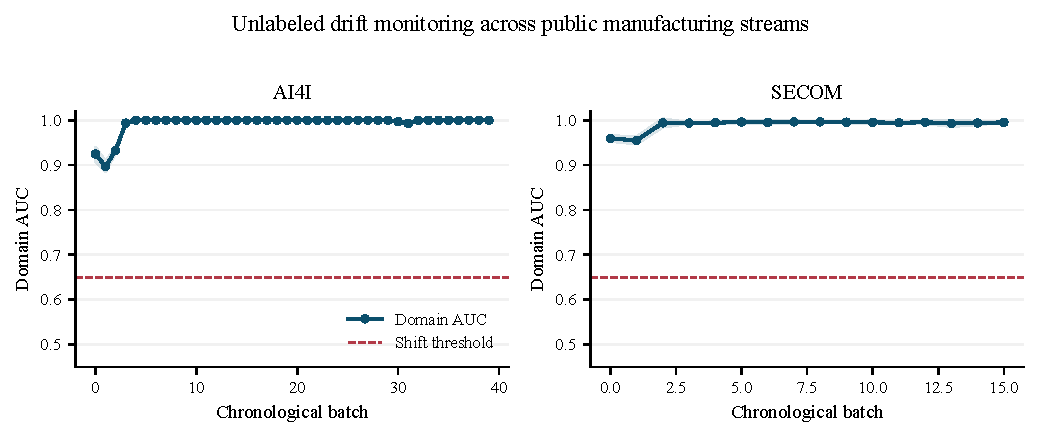
\includegraphics[width=\columnwidth]{figures/drift_monitoring.pdf}
\caption{Cross-fitted domain AUC across the two original chronological streams. The horizontal line is $\gamma=0.65$; shaded bands show seed variation.}
\label{fig:drift}
\end{figure}

\begin{figure}[t]
\centering
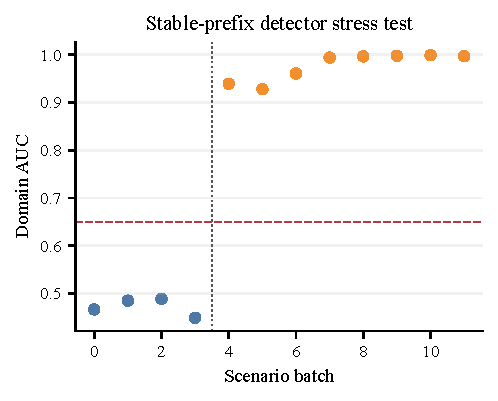
\includegraphics[width=\columnwidth]{figures/stable_prefix_detector.pdf}
\caption{Detector-only stress test with four calibration-like batches followed by an abrupt switch to the original test features. The vertical line separates phases.}
\label{fig:stable}
\end{figure}

\subsection{Sensitivity analysis}
Figure~\ref{fig:sensitivity} and the exported sensitivity CSV files show the one-factor sweeps. On SECOM, DTCG's missed-failure rate remains below 5\% for $\alpha\in\{0.05,0.10\}$ and rises to 8.9\% at $\alpha=0.15$ and 11.3\% at $\alpha=0.20$; auto-release increases from 18.0\% to 35.6\%. On AI4I, $\alpha=0.05$ reduces missed failures to 6.4\% but lowers auto-release to 81.1\%; the default reaches 10.1\% at 88.9\% auto-release.

The $\gamma$ sweep has no effect on the original streams because all observed AUC values are above the largest tested value $0.75$; this is itself evidence that the original data provide little trigger-threshold resolution. Batch size matters more: on SECOM missed failures range from 2.6\% at batch size 25 to 5.6\% at 100, while AI4I ranges from 5.7\% to 13.3\%. Smaller batches react faster but make the domain estimate noisier and increase detector computation. Class weight is consequential on SECOM: $w_1=4$ gives 0.4\% missed failures but only 5.5\% auto-release, whereas $w_1=16$ and 32 raise missed failures to 13.6\% and 15.0\%. AI4I is comparatively insensitive, with 10.1--10.9\% missed failures across the sweep.

\begin{table}[t]
\centering
\caption{Sensitivity ranges across the declared sweeps. Values are ranges of mean rates.}
\label{tab:sensitivity}
\small
\begin{tabular}{lcc}
\toprule
Factor & SECOM missed failure & AI4I missed failure \\
\midrule
$\alpha$ & 3.3--11.3\% & 6.4--10.1\% \\
$\gamma$ & 3.3--3.3\% & 10.1--10.1\% \\
Batch size & 2.6--5.6\% & 5.7--13.3\% \\
Class weight & 0.4--15.0\% & 10.1--10.9\% \\
\bottomrule
\end{tabular}
\end{table}

\begin{figure}[t]
\centering
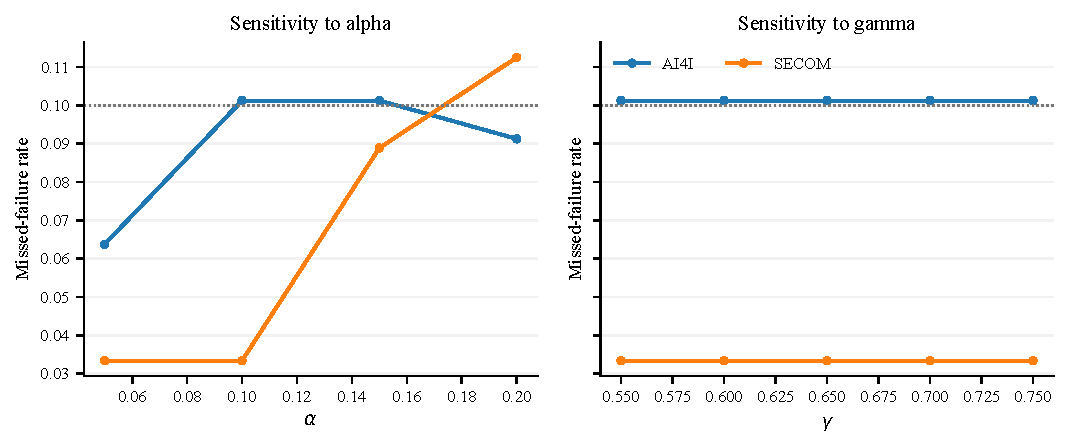
\includegraphics[width=\columnwidth]{figures/sensitivity.pdf}
\caption{Mean missed-failure rate under independent $\alpha$ and $\gamma$ sweeps. The dotted line is the nominal $\alpha=0.10$ reference.}
\label{fig:sensitivity}
\end{figure}

\subsection{Weighted-Mondrian diagnostics}
Weighted-Mondrian obtains 32.8\% auto-release and 10.0\% missed failures on SECOM, and 90.9\% auto-release and 10.1\% missed failures on AI4I. The result is consistent with its target-weighted quantile construction, not evidence of exact validity: the density ratio is estimated by a high-dimensional logistic classifier and clipped to $[0.05,20]$. The diagnostic export shows that low clipping occurs in only a small fraction of calibration points and high clipping is zero in every recorded batch; the limitation is therefore not simply a mass of weights clipped to 20. Rather, the estimated ratios are noisy and the class-specific failure calibration sets are small, especially on SECOM. Weighted-Mondrian trades inspection for nominal-level risk but lacks DTCG's explicit first-shift action and stateful audit semantics.

\begin{figure}[t]
\centering
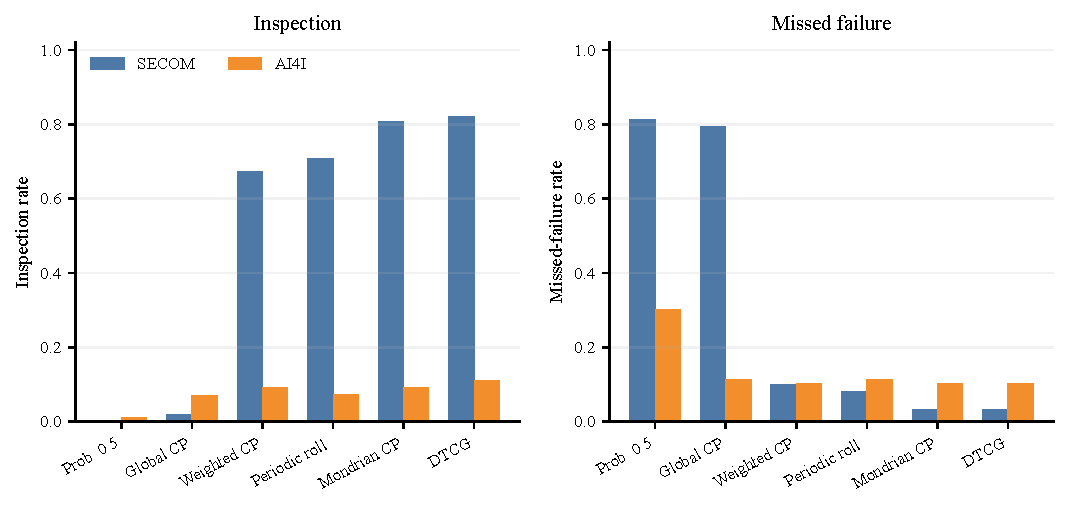
\includegraphics[width=\columnwidth]{figures/gate_performance.pdf}
\caption{Inspection and missed-failure rates for the two public manufacturing streams.}
\label{fig:gate}
\end{figure}

\section{Industrial Implications and Discussion}
\label{sec:discussion}

\subsection{What the experiment supports}
The evidence supports three engineering conclusions. First, overall confidence is not a release policy under rare failures and distribution shift: probability and global CP release almost everything on SECOM while missing most failures. Second, class-conditional calibration is a useful low-complexity safety layer for the public proxy, reducing missed failures to about 3.3\% at the cost of inspecting about 81\% of samples. Third, drift detection is useful only when connected to an action and a state machine. A domain AUC dashboard alone is not a quality control; DTCG turns it into a first-shift hold, delayed-label protocol, and reviewable event.

DTCG's core value relative to Mondrian-CP is not a lower missed-failure rate. The paired tests show no significant missed-failure difference, and both methods produce 3.3\% on SECOM. DTCG adds: (i) an explicit first-shift hold, (ii) a legal-by-construction rule that current labels cannot update current decisions, (iii) rolling calibration only after a minimum number of inspected failures, and (iv) a batch event that ties drift evidence to the quality decision. On the original streams the state counts are 5 first-shift-hold, 10 shifted-base, and 65 shifted-rolling batches for SECOM; AI4I has 5, 20, and 175. These counts quantify that the proposed policy is mostly conservative after the first detected shift, not that it has discovered a new uncertainty theorem.

\subsection{Industrial Implications}
\label{sec:implications}
\begin{enumerate}
    \item \textbf{Deployable decision layer.} DTCG can run after an existing classifier and before a release/inspection router. The domain detector and random forest use standard linear algebra and tree inference, so the architecture does not require a GPU. With $d$ features, the detector fit is approximately linear in the number of calibration-plus-batch rows times $d$ per optimization iteration; the forest inference cost is proportional to the number of trees, tree depth, and batch size. The current implementation has no retraining in the decision loop.
    \item \textbf{Edge resources and latency.} A batch-level detector amortizes its fit across a lot and makes computation predictable. Batch size 25 gives earlier reaction but more detector fits; batch size 100 reduces trigger overhead but can delay escalation and increases missed-failure risk in the sensitivity study. A production service should measure wall-clock latency, memory, and network transfer on the selected edge gateway rather than infer them from public-data runtime.
    \item \textbf{Missing data and sensor outages.} Training-only median imputation is reproducible, but it can mask a failed sensor and create an artificial domain shift. A production implementation should add sensor-health flags, missingness indicators, range checks, stale-value detection, and a fail-safe route for critical sensor outages. The quality gate should never interpret an imputed value as evidence that the sensor was healthy.
    \item \textbf{MES/QMS integration.} The audit event maps to a lot or serial number, model/calibration/policy versions, drift evidence, threshold, auto-release or inspection action, and the final nonconformance disposition. A QMS can retain the human decision; an MES can retain the routing and timestamp; the digital thread can link the event to process, equipment, supplier, and product metadata.
    \item \textbf{Quality-engineer interaction.} The first-shift hold gives an engineer a concrete review queue and an interpretable reason for escalation. The engineer can inspect sensor health, process context, and nonconformance evidence before the policy is allowed to use completed labels. The gate is an aid to quality engineering, not an autonomous authority to release aircraft hardware.
    \item \textbf{Transition to a real line.} The safe path is shadow mode, historical replay across products and suppliers, cost-matrix selection of $\alpha$ and $m$, calibration against real inspection latency, a human override process, and only then a limited release pilot. Airbus-oriented deployment would require de-identified manufacturing data, MES/QMS interfaces, and approval under the applicable quality and safety processes.
\end{enumerate}

\subsection{Weighted baseline and limitations}
The weighted baseline demonstrates why higher release efficiency is not automatically better. Its estimated density ratio is a useful diagnostic but can be unstable in a high-dimensional, small-failure calibration block. DTCG intentionally chooses a more conservative operating point rather than optimizing auto-release alone.

There are six limitations. (1) SECOM is semiconductor data and AI4I is synthetic predictive-maintenance data, so aerospace transfer is unvalidated. (2) The datasets contain one ordered trace each; the failure counts are small in the SECOM test segment, making the batch-level standard deviations wide. (3) The domain classifier detects feature shift but does not identify root cause, label shift, or conditional risk. (4) $\gamma=0.65$, $m=5$, and the batch sizes are engineering settings, not universal optima. (5) Retrospective test labels are available to compute metrics, while a live gate would only see labels for inspected units after delay. (6) The paper does not measure real gateway latency, sensor outage behavior, human override rates, or quality-system integration.

Before industrial use, the method must be validated with multiple product variants, equipment states, suppliers, production-rate regimes, and real inspection dispositions. No automatic release should be enabled solely from the evidence in this paper.

\section{Conclusion}
\label{sec:conclusion}
We presented DTCG, a traceable decision layer for industrial quality and maintenance AI under production shift. It combines an unlabeled domain-AUC trigger, class-conditional conformal calibration, a first-shift inspection hold, delayed-label rolling updates, and a batch-level audit event. On two public manufacturing proxies, naive/global rules missed many failures; class-conditional and DTCG policies reduced the SECOM missed-failure rate to 3.3\%, while AI4I exposed a less conservative but near-nominal 10.1\% regime. Ablations and paired tests show that DTCG should not be sold as quantitatively superior to static Mondrian-CP on missed failures. Its additional value is operational: distribution-shift evidence changes the policy, labels are used only when available, and every state transition is traceable.

\section*{Declarations}
\textbf{Data availability:} The UCI SECOM and AI4I 2020 Predictive Maintenance datasets are publicly available from the UCI Machine Learning Repository under DOI 10.24432/C54305 and DOI 10.24432/C52G8C, respectively.

\textbf{Code and results availability:} The reproducibility package, including \texttt{run\_experiment.py}, frozen result CSV files, figures, and the experiment manifest, is included with this manuscript's supplementary materials. A permanent public GitHub/Zenodo URL and DOI will be attached to the IEEE submission record before publication; the local package is the current review artifact.

\textbf{Funding:} This study received no external funding.

\textbf{Conflict of interest:} The authors declare no competing interests.

\textbf{CRediT authorship contribution:} Siqiang Zhao: Conceptualization, Methodology, Software, Investigation, Data curation, Visualization, and Writing--original draft. Fengxiang Zhang: Validation, Formal analysis, and Writing--review and editing.

\textbf{Generative-AI disclosure:} Generative AI tools were used to assist with language drafting, code refactoring, statistical checks, figure-generation code, and IEEE LaTeX assembly. The authors defined the research question, methods, data protocol, thresholds, and claim boundaries; reran and inspected the experiments; verified the numerical statements and citations; and take full responsibility for the manuscript.

\textbf{Ethical and safety statement:} The experiments use public, non-personal datasets. The proposed gate is not validated for autonomous release of safety-critical aerospace hardware; real deployment requires quality-engineering and safety approval.

\bibliographystyle{IEEEtran}
\bibliography{references}

\end{document}
